\documentclass[../main.tex]{subfiles}
\graphicspath{{img},{img/ink},{ink}}

\begin{document}

\begin{tcolorbox}[
    width=\textwidth,
    height=\textheight,
    title=Phyphox: Kraft und Druck,
    fonttitle=\Large,
    before title=\vspace{0.2cm}, after title=\vspace{0.2cm},
    colback=white,
    title filled=true, 
    colbacktitle=myorange,
    colframe=black,
    coltitle=black,
    ]

    \vspace{0.2cm}
    \textbf{Klassenstufe}: 9/10

    \vspace{0.4cm}

    \textbf{Fachlicher Bezug}: Zusammenhang Druck - Kraft / Druck - Fläche, Einheit Pascal

    \vspace{0.2cm}
    \begin{minipage}[]{0.5\textwidth}


        \textbf{Material}: 
        \begin{itemize}[noitemsep]
            \item Gefrierbeutel (evtl. zusätzlich Gummiband)
            \item 2 Handys + Phyphox 
            \item Behälter oder dünne Unterlage 
            \item verschiedene Massestücke 
        \end{itemize}


    \end{minipage}
    \hspace{1.2cm}
    \begin{minipage}[]{0.45\textwidth}
        \vspace{0.2cm}
        \includegraphics[width=0.9\textwidth]{img/versuchsaufbau}
    \end{minipage}

    \vspace{0.4cm}
    \textbf{Aufbau}: In der Phyphox-App wird unter dem Reiter \glqq Sensoren\grqq{} die Auswahl \glqq Luftdruck\grqq{} getroffen. Im Experiment wird dann in den Tabs \glqq Einfach\grqq{} ausgewählt. Der Fernzugriff wird gestartet. Das Handy wird in den Gefrierbeutel gelegt, etwas Luft wird hineingepustet und gut verschlossen. Ein Behälter, zum Auflegen der Massestücke, wird sicher auf dem Beutel platziert. In einem zweiten Handy werden die Messwerte des Luftdrucks über den Fernzugriff abgelesen.  

    \vspace{0.4cm}
    \textbf{Durchführung}: 
    \begin{enumerate}
        \item \textbf{Druckänderung in Abhängigkeit von der wirkenden Kraft} \\
            Zunächst wird der Ausgangswert des Luftdrucks $p_{L_1}$ \underline{mit} Behälter und \underline{ohne} Massestück notiert. Es werden dann nacheinander verschiedene Massen $m$ aufgelegt. Die Kraft $F = m \cdot g$ wird berechnet. Aus dem neuen Luftdruck $p_L$ bestimmt man den Druck $p = p_L - p_{L_1}$ (in der Einheit hPa) infolge der zusätzlichen Kraft. Die Werte werden in eine Tabelle und Koordinatensystem eingetragen.
        \item \textbf{Abhängigkeit des Drucks von der Fläche}\\
            Zunächst wird der Ausgangswert des Luftdrucks $p_{L_2}$ \underline{ohne} Behälter und \underline{ohne} Massestück festgehalten. Im ersten Durchgang wird ein Massestück in den Behälter gelegt und die Druckänderung notiert. Im zweiten Durchgang liegt dasselbe Massestück unten und der Behälter wird durch leichtes Stützen darauf balanciert.  

    \end{enumerate}

    \vspace{0.4cm}
    \textbf{Ergebnis}: 
    \begin{enumerate}
        \item Die Auflagefläche ist für alle Massestücke identisch. Man beobachtet die Proportionalität
            \begin{align*}
                p \sim F
            \end{align*}
        \item Man beobachtet, dass der Druck bei kleinerer Auflagefläche stärker zunimmt. Darüber lässt sich die Formel
            \begin{align*}
                p = \frac{F}{A}
            \end{align*}
            motivieren.
    \end{enumerate}

\end{tcolorbox}


\end{document}
